\documentclass[t]{beamer}
\usepackage{CJKutf8}
\usepackage{amsfonts}
    \usepackage{amsmath}
    \usepackage{amssymb}
    \usepackage{amsthm}
    \usepackage{enumerate}
    \usepackage{graphicx}
    \usepackage{layout}
    \usepackage{mathrsfs}
    \usepackage{fancyhdr}
    \usepackage{subfigure}
    \usepackage{tcolorbox}
    \usepackage{tikz-cd}
    \usepackage{color}
    \usepackage{pifont}
    \usepackage{verbatim}
    \usepackage{mathtools}
    \usepackage{float}
    \usepackage{bm}
    \usetheme{AnnArbor}
% \usetheme{Antibes}
\usecolortheme{beaver}
\usepackage{listings}

% 设置JSON样式
\lstdefinestyle{json}{
    basicstyle=\tiny\ttfamily,
    columns=fullflexible,
    showstringspaces=false,
    commentstyle=\color{gray},
    keywordstyle=\color{blue},
    stringstyle=\color{red},
    breaklines=true,
    frame=single,
    captionpos=b,
    aboveskip=10pt,
    belowskip=10pt
}

\lstset{
    language=Python, % 设置代码块语言为Python
    breaklines=true, % 自动换行
    basicstyle=\small\ttfamily, % 设置基本字体样式
    keywordstyle=\bfseries\color{blue}, % 设置关键字样式
    commentstyle=\itshape\color{gray}, % 设置注释样式
    showstringspaces=false, % 不显示字符串中的空格
    frame=single, % 设置代码块边框样式
    numbers=left, % 行号显示在左侧
    numberstyle=\tiny\color{gray}, % 设置行号样式
    stepnumber=1, % 设置行号间隔
    tabsize=4 % 设置制表符宽度
}


% 设置shell样式
\lstdefinestyle{shell}{
    language=bash,
    basicstyle=\tiny\ttfamily,
    columns=fullflexible,
    showstringspaces=false,
    commentstyle=\color{gray},
    keywordstyle=\color{blue},
    stringstyle=\color{red},
    breaklines=true,
    frame=single,
    captionpos=b,
    aboveskip=10pt,
    belowskip=10pt
}

\usepackage{subfigure}

% 添加网址的命令
\usepackage{hyperref}
% 这是一个带链接文本的示例:\href{https://www.example.com}{点击这里访问网站}
% 普通的示例:\url{https://www.example.com}
% 表格
\usepackage{booktabs}
\usepackage{multirow}

% \setbeamertemplate{navigation symbols}{}

\usepackage{textpos}

\newcommand{\dif}{\mathrm{d}}
\newtheorem{thm}{{定理}}

% some common command
\newcommand{\mm}[1]{$ #1$\newline}
% \newcommand{\tuichu}{\Rightarrow}
% \newcommand{\li}[1]{\newline#1}



\newcommand{\analysis}[2]{\forall \mathcal{E}{#1},\exists \delta {#2},s.t.}
\newcommand{\denyanalysis}[2]{\exists \mathcal{E}{#1},\forall \delta {#2},s.t.}
\newcommand{\yield}{\Rightarrow }
\newcommand{\jj}{\newline}
\newcommand{\ff}[1]{$ #1$}   % math environment + newline
\newcommand{\fgn}[1]{\begin{equation}#1\end{equation}  }
\newcommand{\fg}[1]{$$ #1$$}   % math environment + newline 
\newcommand{\pf}{$proof.$\newline}
\newcommand{\ee}{\newline\ff{\Box}\newline}
\newcommand{\fenshi}[2]{\ff{\frac{#1}{#2}}}
\newcommand{\shenlue}{\vdots\jj}
\newcommand{\abs}[1]{{\left \lvert #1 \right\rvert}}
\newcommand{\loge}[1]{In ({#1})}
\newcommand{\logical}[2]{log_{#2}^{#1}}
\newcommand{\summary}[3]{$\sum_{{#1}={#2}}^{#3}  $}
\newcommand{\denjia}[2]{{#1}\Leftrightarrow {#2}}
\newcommand{\jihe}[3]{ {#1}  = \{ {#2} \mid {#3} \} }
\newcommand{\ve}[2]{\left\langle {#1},{#2}\right \rangle}
\newcommand{\dakuohao}[2]{\begin{array}{rcl}{#1}\end{array} \} \Rightarrow{#2}}
\newcommand{\sxb}[3]{#1^{#2}_{#3}}
\newcommand{\sss}[2]{#1^{#2}}
\newcommand{\xxx}[2]{#1_{#2}}
\newcommand{\bri}[1]{\uppercase\expandafter{\romannumeral#1}}
\newcommand{\ri}[1]{\romannumeral#1} 
\newcommand{\polynomial}[8]{#1_{#2}#6^{#7}+#1_{#3}#6^{#8}+...+#1_{#4}#6+#1_{#5} }
\newcommand{\newd}[4]{f[{#1}_{#2},{#4},{#1}_{#3}]}
\newcommand{\lb}[2]{\begin{align*}\begin{split}{#1}\{ {#2}\end{split}\end{align*}}
\newcommand{\tab}[1]{\begin{array}{ll} {#1}\end{array}}


% 向量乘积
\newcommand{\avg}[1]{\left\langle #1 \right\rangle}
% 偏微分方程
\newcommand{\difFrac}[2]{\frac{\dif #1}{\dif #2}}
\newcommand{\pdfrac}[2]{\frac{\partial{#1}}{\partial{#2}}}
% 不同章节
\newcommand{\one}[1]{\section{#1}}
\newcommand{\two}[1]{\subsection{#1}}
\newcommand{\three}[1]{\subsubsection{#1}}
\newcommand{\aone}[1]{\section*{#1}}
\newcommand{\atwo}[1]{\subsection*{#1}}
\newcommand{\athree}[1]{\subsubsection*{#1}}
% 大括号,左右都有
\newcommand{\lbra}[1]{\left\{  {\begin{matrix} #1 \end{matrix}}\right. } 
% 样式 括号前缀 + 括号 
\newcommand{\lbras}[2]{{#1}\left\{ {  {\begin{matrix} #2 \end{matrix}}}\right. } 
\newcommand{\rbra}[1]{ \left.  {\begin{matrix} #1 \end{matrix}} \right\}  } 
% 模长
\newcommand{\distance}[1]{\parallel #1\parallel }
% 等价
\newcommand{\equ}{\Longleftrightarrow }
% 共轭
\newcommand{\cja}[1]{\overline{#1}}
% 两个矩阵,上面是 方框[] 下面是线条| 中间是 无
\newcommand{\mtx}[1]{\begin{matrix}#1\end{matrix} }
\newcommand{\bmtx}[1]{\begin{bmatrix}#1\end{bmatrix} }
\newcommand{\vmtx}[1]{\begin{vmatrix}#1\end{vmatrix} }
% \newcommand{\table}[1]{\begin{array}[lr]{ccc} #1 \end{array}}

%输入普通字符
\newcommand{\ww}[1]{\text{#1}}

% 所有内容 直接头文件搞定
\newcommand{\everything}[1]{\begin{document}\begin{CJK*}{UTF8}{gkai}#1\end{CJK*}\end{document}}


% 存放代码(失败了)
\newcommand{\cccode}[1]{\begin{lstlisting}#1\end{lstlisting}}

% 改变特定行序列
\newcommand{\ttt}{\subsection{}}

% 嵌套序号
\newcommand{\eee}[1]{\begin{enumerate}#1\end{enumerate}}


% 模板里面的一些宏
\newcommand{\pdfFrac}[2]{\frac{\partial #1}{\partial #2}}
\newcommand{\OFL}{\mathrm{OFL}}
\newcommand{\UFL}{\mathrm{UFL}}
\newcommand{\fl}{\mathrm{fl}}
\newcommand{\op}{\odot}
\newcommand{\Eabs}{E_{\mathrm{abs}}}
\newcommand{\Erel}{E_{\mathrm{rel}}}
% 变化颜色
\newcommand{\red}{\textcolor{red}}
\newcommand{\blue}{\textcolor{blue}}
% 注释代码
% \newcommand{\undef}[1]{\iffalse #1 \fi}

% 流程图需要用到的宏包
\usepackage{palatino}
\usepackage{tikz}
\usetikzlibrary{shapes.geometric, arrows}
\tikzstyle{startstop} = [rectangle, rounded corners, minimum width = 2cm, minimum height=1cm,text centered, draw = black, fill = red!40]
\tikzstyle{io} = [trapezium, trapezium left angle=70, trapezium right angle=110, minimum width=2cm, minimum height=1cm, text centered, draw=black, fill = blue!40]
\tikzstyle{process} = [rectangle, minimum width=3cm, minimum height=1cm, text centered, draw=black, fill = yellow!50]
\tikzstyle{decision} = [diamond, aspect = 3, text centered, draw=black, fill = green!30]
% 箭头形式
\tikzstyle{arrow} = [->,>=stealth]
% 4个非常重要 的新命令
\newcommand{\start}[2]{    \node (start) [startstop]{#1};\node (in1) [io, below of = start]{#2};\lin{start}{in1}{}}
\newcommand{\stopp}[3]{\node (out1) [io, below of= #1]{#2};\node (stop) [startstop, below of=out1]{#3};\lin{out1}{stop}{} }
\newcommand{\pro}[6]{    \node (#3) [process, #2 of=#1,xshift=#4 cm]{#5};}
\newpage
\newcommand{\lin}[3]{\draw [arrow] (#1) --node [above] {#3} (#2);}


\begin{document}
\begin{CJK*}{UTF8}{gkai}
% 一般第一页显示PPT标题以及作者信息

% \BackgroundPic{./Screenshot from 2022-04-20 16-31-08.png}

% 增加学校 前面
\addtobeamertemplate{title page}{}{
	\begin{tikzpicture}[remember picture,overlay]
		% \node[yshift=85pt,xshift=50pt]{\includegraphics[height=2cm]{Screenshot from 2022-04-20 16-51-21.png}};
\end{tikzpicture}
}
	% \title{时间序列数据集}
	\title{组会汇报}
	\subtitle {} %不需要
	\author{
		陈钶杰\, \\
		专业:计算数学\,
	} % 显示作者
	% \institute {学院:数学科学学院} % 设置学院机构	
	\date{\today}  % 显示日期
\titlepage

% 设置目录
\begin{frame}{目录}
\frametitle{目录}	
\tableofcontents  % 显示目录
\end{frame}


\section{代码调试}

\begin{frame}
    \frametitle{时间序列模型与自然语言模型对比实验}
    \eee{
        \item 将50支股票分别选取6支并做对比实验
        \item 进行可视化对比语言模型和时间序列模型的对比
        \item 线性模型的指标对比中,对数据进行四舍五入。
    }
\end{frame}


\begin{frame}
    \frametitle{评估指标}
    \small
    \eee{
        \item 准确率:准确率是模型正确分类的样本数与总样本数之比。它衡量了模型的整体性能,但在不平衡类别分布的情况下可能不是一个很好的指标。
        \item 宏平均精确度:它计算每个类别的精确度,然后取平均值。不考虑类别不平衡,对每个类别的性能平等看待。
        \item 宏平均召回率:与宏平均精确度类似,它计算每个类别的召回率,然后取平均值。也不考虑类别不平衡,对每个类别的性能平等看待。
        \item 宏平均F1分数:它计算每个类别的F1分数,然后取平均值。对每个类别的性能平等看待,适用于类别不平衡的问题。
        \item 微平均精确度:它计算所有类别的真正例和假正例的总数,然后计算总的精确度。在类别不平衡时,它更受到正例类别的影响。
        \item 微平均召回率:它计算所有类别的真正例和假负例的总数,然后计算总的召回率。也在类别不平衡时受到正例类别的影响。
        \item 微平均F1分数:它计算所有类别的真正例、假正例和假负例的总数,然后计算总的F1分数。同样,它在类别不平衡时受到正例类别的影响。
% \item 分类报告(Classification Report):分类报告通常包括每个类别的精确度、召回率、F1分数等指标,以及这些指标的宏平均和微平均值。
    }
\end{frame}

\subsection{对测试集数据进行预测,并计算预测误差}

\begin{frame}

    \begin{table}[ht]
        \centering
        \caption{准确率结果}
        \tiny
        \label{tab:example}
        \begin{tabular}{|c|l|r|c|c|c|}
        \hline
        sss   & chatglm & DLinear(one/much) & Autoformer(one/much)  & Informer(one/much)  & Transformer(one/much) \\
        \hline
        样例1 & \red{0.16} & 0.0021/0.0 & 0.1203/0.1266  & 0.1701/0.0  & 0.1701/0.029\\
        \hline
        样例2 & \red{0.1684} &0.0021/0.0  &0.1245/0.1203  &0.1743/0.0   & 0.1743/0.029\\
        \hline
        样例3 & \red{0.8877} & 0.0/0.0 & 0.4772/0.3672  & 0.7573/0.0  & 0.187/0.0332\\
        \hline
        样例4 & \red{0.158} & 0.0/0.0 & 0.1037/0.11  & 0.1556/0.0  &0.1701/0.029 \\
        \hline
        样例5 & \red{0.1601} & 0.0083/0.0 & 0.1017/0.0975  & 0.0996/0.0  & 0.1058/0.0436\\
        \hline
        样例6 & \red{0.2869} & 0.0/0.0 &  0.0166/0.0145 & 0.0041/0.0  & 0.0041/0.0041\\
        \hline
    \end{tabular}
        \end{table}
            

\end{frame}

\subsection{预测结果可视化}

\begin{frame}
    \frametitle{\tiny 使用一个时间序列模型进行训练}    
    \begin{figure}[ht]
        \centering
        \subfigure[测试例1]{
            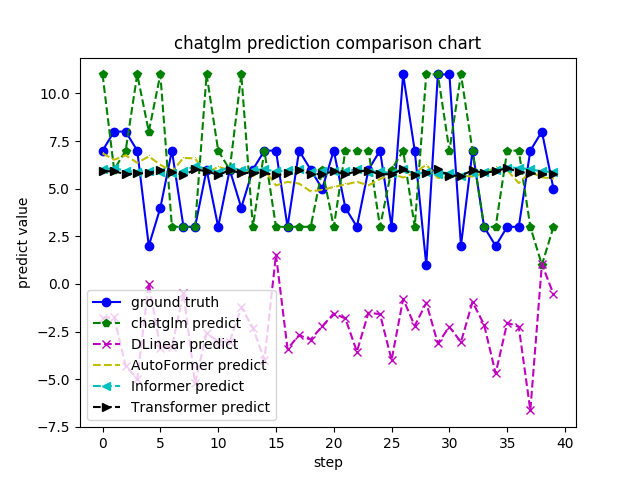
\includegraphics[width=0.45\textwidth]{png/png_one/01.png}
        }
        \hfill
        \subfigure[测试例2]{
            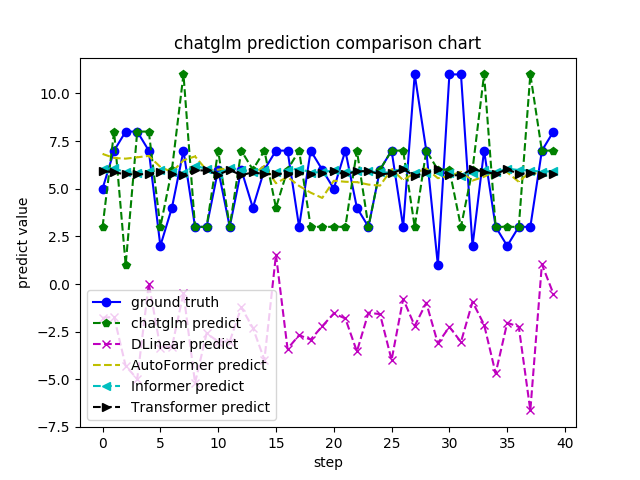
\includegraphics[width=0.45\textwidth]{png/png_one/02.png}            
        }
    \end{figure}
\end{frame}

\begin{frame}
    \frametitle{\tiny 使用一个时间序列模型进行训练}    
    \begin{figure}[ht]
        \centering
        \subfigure[测试例3]{
            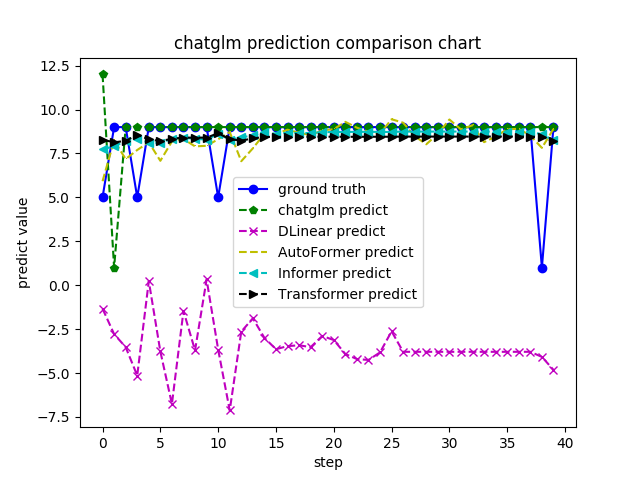
\includegraphics[width=0.45\textwidth]{png/png_one/03.png}
        }
        \hfill
        \subfigure[测试例4]{
            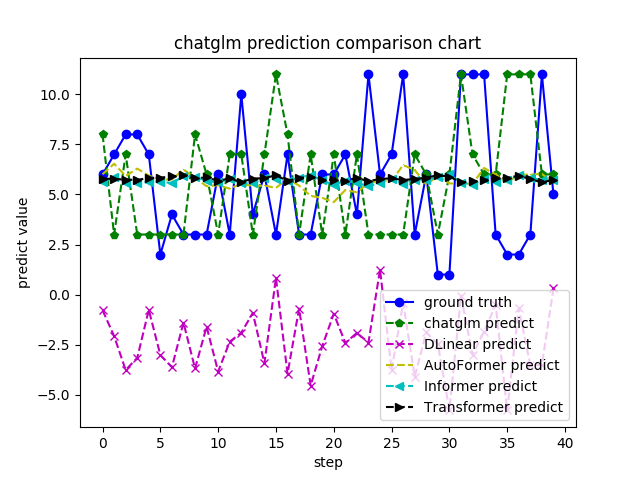
\includegraphics[width=0.45\textwidth]{png/png_one/04.png}            
        }
    \end{figure}
\end{frame}

\begin{frame}
    \frametitle{\tiny 使用一个时间序列模型进行训练}    
    \begin{figure}[ht]
        \centering
        \subfigure[测试例5]{
            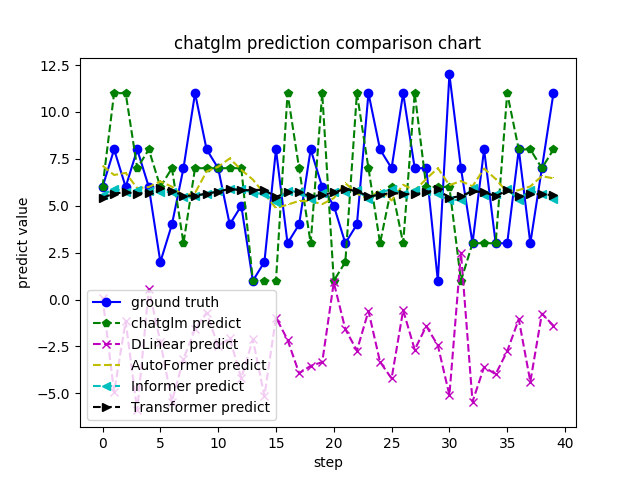
\includegraphics[width=0.45\textwidth]{png/png_one/05.png}
        }
        \hfill
        \subfigure[测试例6]{
            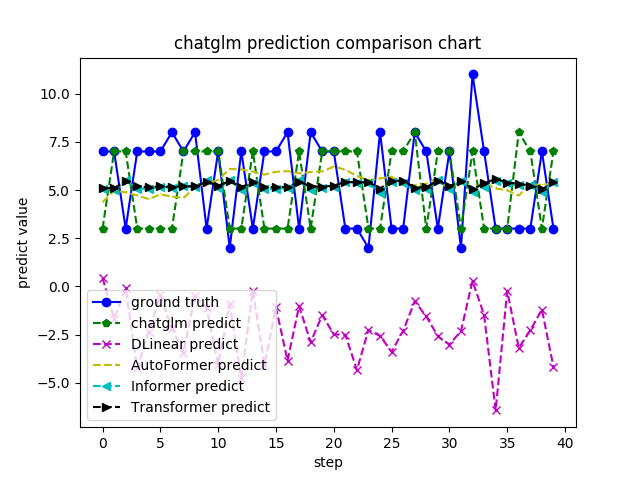
\includegraphics[width=0.45\textwidth]{png/png_one/06.png}            
        }
    \end{figure}
\end{frame}


\begin{frame}
    \frametitle{\tiny 使用多个时间序列模型进行训练}    
    \begin{figure}[ht]
        \centering
        \subfigure[测试例1]{
            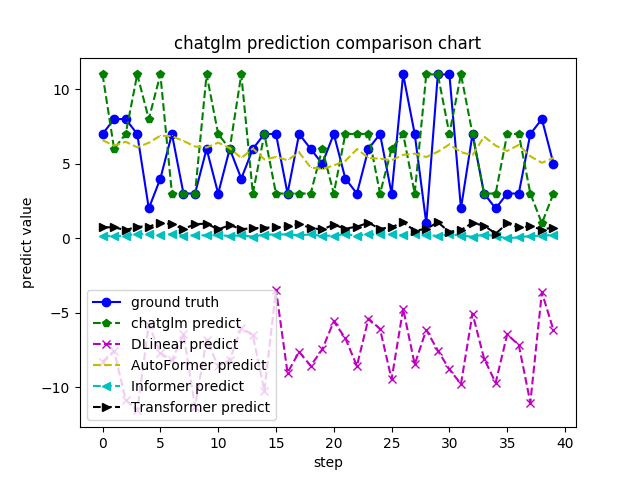
\includegraphics[width=0.45\textwidth]{png/png_two/01.png}
        }
        \hfill
        \subfigure[测试例2]{
            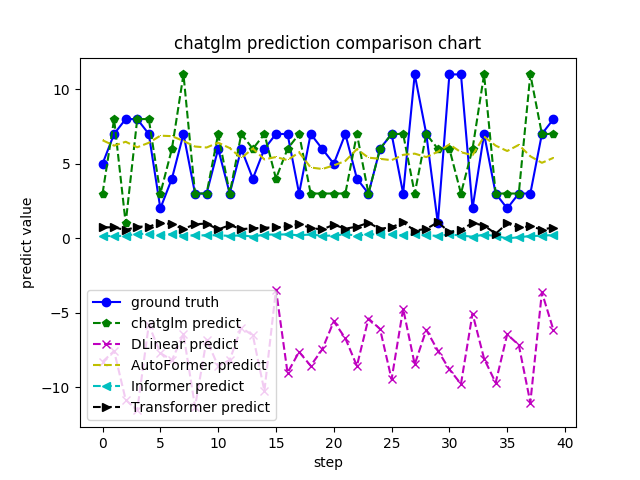
\includegraphics[width=0.45\textwidth]{png/png_two/02.png}            
        }
    \end{figure}
\end{frame}

\begin{frame}
    \frametitle{\tiny 使用多个时间序列模型进行训练}    
    \begin{figure}[ht]
        \centering
        \subfigure[测试例3]{
            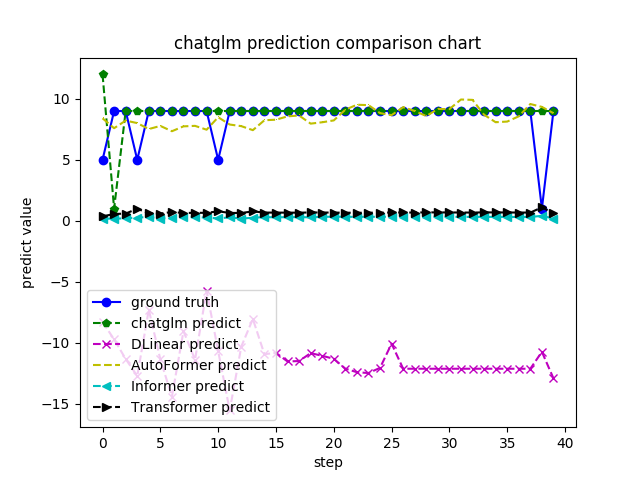
\includegraphics[width=0.45\textwidth]{png/png_two/03.png}
        }
        \hfill
        \subfigure[测试例4]{
            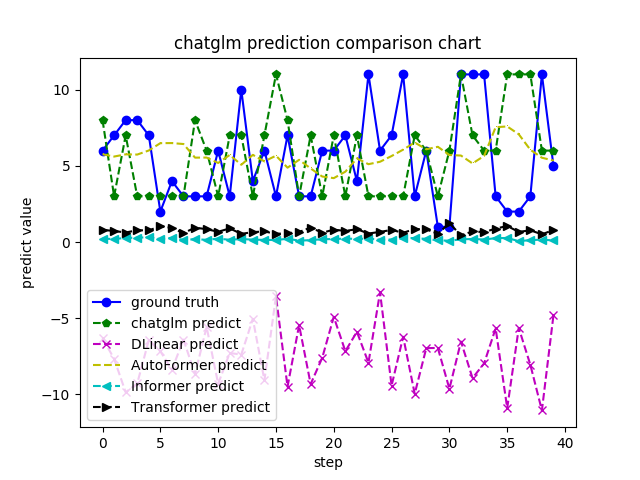
\includegraphics[width=0.45\textwidth]{png/png_two/04.png}            
        }
    \end{figure}
\end{frame}


\begin{frame}
    \frametitle{\tiny 使用多个时间序列模型进行训练}    
    \begin{figure}[ht]
        \centering
        \subfigure[测试例5]{
            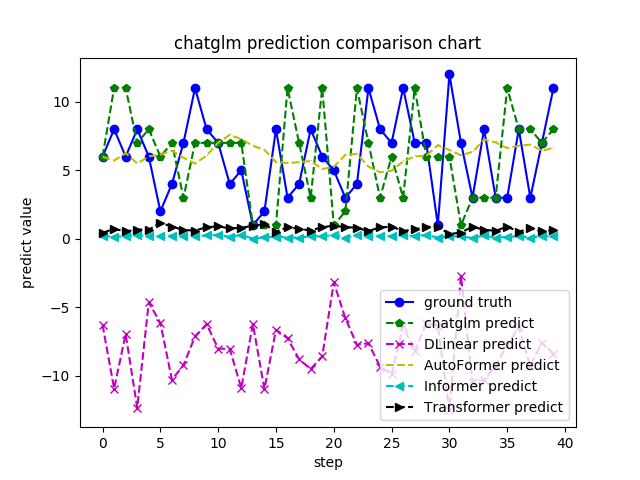
\includegraphics[width=0.45\textwidth]{png/png_two/05.png}
        }
        \hfill
        \subfigure[测试例6]{
            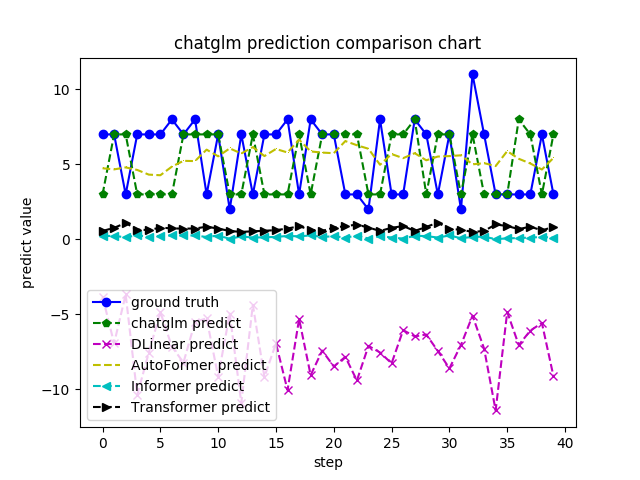
\includegraphics[width=0.45\textwidth]{png/png_two/06.png}            
        }
    \end{figure}
\end{frame}




% \begin{frame}
%     \frametitle{k-线图结果预测,分别用序列数字代替}
%     % \item k线图一共有12种形式,分别用数字表示1,2,3,4,5,6,7
%     \eee{
%         \item 阴线,上影线: 开盘价高于收盘价,有较长的上影线。
%         \item 阴线,下影线: 开盘价高于收盘价,有较长的下影线。
%         \item 阴线,上下影线: 开盘价高于收盘价,有较长的上影线和下影线。
%         \item 阴线: 开盘价高于收盘价,没有或很短的影线。
%         \item 阳线: 开盘价低于收盘价,没有或很短的影线。
%         \item 阳线,上影线: 开盘价低于收盘价,有较长的上影线。  
%         \item 阳线,下影线: 开盘价低于收盘价,有较长的下影线。
%         \item 阳线,上下影线: 开盘价低于收盘价,有较长的上影线和下影线。
%         \item 阳线,十字影线: 开盘价低于收盘价,有较长的十字影线。
%         \item 阴线,十字影线: 开盘价高于收盘价,有较长的十字影线。        
%         \item 十字阳线: 开盘价等于收盘价,有较长的上影线和下影线。
%         \item 十字阴线: 开盘价等于收盘价,有较长的上影线和下影线。
%     }
% \end{frame}

\begin{frame}
	\frametitle{k线图相关结论}
	\begin{itemize}
        \item 经过多种模型测试,语言模型的准确率均是最高的
        \item 对于分类任务的序列预测,语言模型要优于时间序列模型,而且语言模型还具有强大的泛化能力。
	\end{itemize}
\end{frame}




% \subsection{下一步的计划}
% \begin{frame}
% 	\frametitle{下一步计划及相关问题}	
% 	\begin{itemize}
%         % \item 使用auto-cot,对比当前的结果
%         % \item 能否将RevIN 增加中间步骤提高结果的精确性。        
%         % \item 提取模型中的注意力权重,查看模型对于输入信息的处理细节
%         % \eee{
%         %     \item 如何解决经过规范化以后数值比较接近的问题?
%         % }
% 	\end{itemize}
% \end{frame}

% 结束语
\section{}
\begin{frame}
	\frametitle{}
	\begin{center}
		\Huge{谢谢老师和同学们的聆听!}
	\end{center}
\end{frame}

\end{CJK*}
\end{document}
